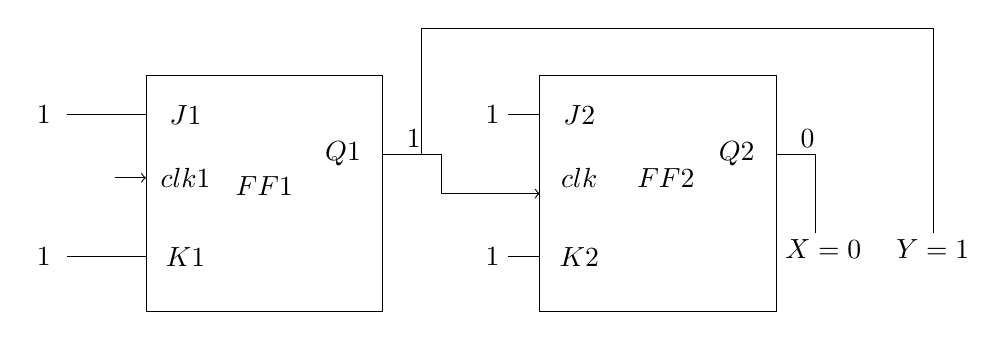
\begin{tikzpicture}
        \draw (2,2) rectangle (5,5);            
        \draw (2.5,2.7) node{$K1$};
        \draw (2.5,3.7) node{$clk1$};
        \draw[->] (1.6,3.7) -- (2,3.7) node[left] {};%connection of clock 1 
        \draw (2.5,4.5) node{$J1$};
        \draw (2,2.7) -- (1,2.7); % this is the connection K
        \draw (0.7,2.7) node{$1$}; % 1 is the given value of K
        \draw (2,4.5) -- (1,4.5); % this the connection of J
        \draw (0.7,4.5) node{$1$}; % 1 is the given value of J
        \draw (5,4) -- (5.75,4);     
        \draw (5.75,4) -- (5.75,3.5);
        \draw (3.5,3.6) node{$FF1$};
        \draw[->] (5.75,3.5) -- (7,3.5) node[left] {};% clock pulse from Q1 to FF2's clock
        \draw (10,4) -- (10.5,4); % this is the connection from Q2
        \draw (5.5,4) -- (5.5,5.6);
        \draw (5.5,5.6) -- (12,5.6);
        \draw (12,5.6) -- (12,3); % this the connection of Y
        \draw (11.99,2.8) node{$Y=1$}; % this is the co-ordinates Y 
        \draw (10.5,4) -- (10.5,3); %this the line of X
        \draw (10.6,2.8) node{$X=0$}; %this is co-ordinates of X
        \draw (4.5,4) node{$Q1$}; % FF1's Q1
        \draw (5.4,4.2) node{$1$}; % 1 is the value of Q1
        \draw (7,2) rectangle (10,5);       
        \draw (7.5,2.7) node{$K2$};   
        \draw (7,2.7) -- (6.59,2.7); % this the connection of k of FF2
        \draw (6.4,2.7) node{$1$}; % 1 is the given value of K of FF2
        \draw (7.5,3.7) node{$clk$}; 
        \draw (8.6,3.7) node{$FF2$};
        \draw (7.5,4.5) node{$J2$};
        \draw (6.4,4.5) node{$1$};
        \draw (7,4.5) -- (6.6,4.5); % this the connection of J of FF2
        \draw (9.5,4) node{$Q2$};
        \draw (10.4,4.2) node{$0$};
        
        
\end{tikzpicture}
